\RequirePackage{amsmath}
\documentclass[twocolumn, times]{aastex631}
\usepackage[spanish,es-minimal,english]{babel}
\usepackage[utf8]{inputenc}
\usepackage{natbib}
%\usepackage{microtype}
\usepackage{hyperref}
\usepackage{savesym}
\savesymbol{tablenum}
\usepackage{siunitx}
\restoresymbol{SIX}{tablenum}
\usepackage[varg]{newtxmath}
\usepackage{newtxtext}
\usepackage{booktabs}
\usepackage{array}   % for \newcolumntype macro
\newcolumntype{L}{>{$}l<{$}} % math-mode version of lrc column types
\newcolumntype{R}{>{$}r<{$}} 
\newcolumntype{C}{>{$}c<{$}} 

\bibliographystyle{aasjournal}

\newcommand\ION[2]{#1\,\scalebox{0.9}[0.8]{\uppercase{#2}}}
\newcounter{ionstage}
\renewcommand{\ion}[2]{\setcounter{ionstage}{#2}% 
  \ensuremath{\mathrm{#1\,\scriptstyle\Roman{ionstage}}}}
\newcommand\hii{\ion{H}{2}}
\newcommand\hi{\ion{H}{1}}
\newcommand\heii{\ion{He}{2}}
\newcommand\hei{\ion{He}{1}}
\newcommand\siii{[\ion{S}{3}]}
\newcommand\sii{[\ion{S}{2}]}
\newcommand\oiii{[\ion{O}{3}]}
\newcommand\ariii{[\ion{Ar}{3}]}
\newcommand\ariv{[\ion{Ar}{4}]}
\newcommand\ARIV{[\ION{Ar}{iv}]}
\newcommand\Raman{\ensuremath{_{\text{Raman}}}}
\def\th#1#2{\(\theta^{#1}\)\,Ori~#2}
\newcommand\wn{\ensuremath{\tilde{\nu}}}
\newcommand\Wav[1]{\ensuremath{\lambda #1}}

% Chemical formulae
\newcommand*\chem[1]{\ensuremath{\mathrm{#1}}}
% Atomic term symbols
\newcommand\Config[1]{\ensuremath{\mathrm{#1}}}
\newcommand\Term[3]{\ensuremath{\mathrm{#1\ ^{#2}#3}}}
\newcommand\Level[4]{\ensuremath{\mathrm{#1\ ^{#2}#3_{#4}}}}

\newcommand\ha{\ensuremath{\text{H}\alpha}}
\newcommand\hb{\ensuremath{\text{H}\beta}}
\newcommand\lya{\ensuremath{\text{Ly}\alpha}}
\newcommand\lyb{\ensuremath{\text{Ly}\beta}}

\newcommand{\wind}{\ensuremath{_{\text{w}}}}
\newcommand\snrj{SNR~J\num{0059.4}\num{-7210}}

\begin{document}
\title{Shielded from the wind: evaporating neutral globules around a Wolf-Rayet star}
\shorttitle{Evaporating globules around WR~124}
\author[0000-0000-0000-0000]{Roberto Reyes-Cabañas}
\affiliation{%
  \foreignlanguage{spanish}{Instituto de Radioastronomía y
    Astrofísica, Universidad Nacional Autónoma de México, Apartado
    Postal 3-72, 58090 Morelia, Michaoacán, Mexico}
}

\author[0000-0001-6208-9109]{William J. Henney}
\affiliation{%
  \foreignlanguage{spanish}{Instituto de Radioastronomía y
    Astrofísica, Universidad Nacional Autónoma de México, Apartado
    Postal 3-72, 58090 Morelia, Michaoacán, Mexico}
}
\email{w.henney@irya.unam.mx}
\correspondingauthor{William J. Henney}


\author[0000-0002-5456-4472]{S. Jane Arthur}
\affiliation{%
  \foreignlanguage{spanish}{Instituto de Radioastronomía y
    Astrofísica, Universidad Nacional Autónoma de México, Apartado
    Postal 3-72, 58090 Morelia, Michaoacán, Mexico}
}

% \author[0000-0002-5406-0813]{Jesús A. Toalá}
% \affiliation{%
%   \foreignlanguage{spanish}{Instituto de Radioastronomía y
%     Astrofísica, Universidad Nacional Autónoma de México, Apartado
%     Postal 3-72, 58090 Morelia, Michaoacán, Mexico}
%   }

\begin{abstract}
  The circumstellar nebula M1-67 around the Wolf-Rayet star WR~124
  contains hundreds of small neutral globules, as revealed by JWST images.
  However, despite the powerful stellar wind from the star, the globules
  do not interact directly with the wind.
  Instead, they are hydrodynamically shielded by a transonic warm ionized
  flow away from their surfaces that is induced by the Lyman continuum radiation
  of the star.
  This inwardly directed photoevaporation flow shocks against the
  outflowing stellar wind to form dense hemispherical ionized shells
  that are a few times larger than the globules
  and which contribute a significant fraction of the recombination line luminosity
  of the nebula.
  We analyze archival HST images of the nebula and estimate the size, brightness,
  and ionized density of each photoevaporation flow and accompanying interaction shell.
  We show that \textit{something, something, something, \dots}.
  We compare the globule-wind interaction around WR~124 with similar interactions
  seen elsewhere, such as photoevaporating disks (proplyds) in the Orion Nebula.
\end{abstract}

\keywords{Circumstellar matter; Stars: winds, outflows}

%\object{M42}

\section{Introduction}
\label{sec:introduction}

\subsection{Glóbulos y sus flujos fotoevapoorativos}
Los glóbulos son concentraciones densas de gas neutro y polvo que se pueden encontrar tanto en regiones de formación estelar como en nebulosas alrededor de estrellas evolucionadas, por lo que tenemos una gran vcariedad de tamaños (1--\SI{e-2}{pc}). Estos góbulos se pueden formar poro colapso gravitacional, inestabilidades térmicas o turbulencia. Generalmente se le suele llamar nudos a los glóbulos que se encuentran en nebulosas circunestelares, y suelen ser las de menor tamaño ($\leq$\SI{e-2}{pc}).

Las estrellas Wolf-Rayet son estrellas masivas evolucionadas que tienen una gran perdida de masa debido a su gran viento solar lo que produce una nebulosa a su alrededor. En las recientes imagenes del JWST, se ha podido apreciar con gran detalle la presencia de grumos en la nebulosa circumestellar en M1-67. Estos grumos son globulos moleculares neutros que tienen una gran densidad y pueden ser principalmente de hidrogeno neutro. 

Cuando los glóbulos interactúan con la radiación ionizante de una estrella jóven masiva, este comienza a ionizar el glóbulo, provocando que un flujo de partículas ionizadas viajen en dirección a la estrella, este es conocido como flujo fotoevaporativo (). \textbf{falta decir acerca de las condiciones de la EM para que no ionizar todo el glóbulo y decir lo de equilibrio de ionización}.

\subsection{Estrellas WR}

Las estrellas Wolf-Rayet (WR) son estrellas evolucionadas que se caracterizan por tener intensas líneas de eimisión de  He, C, O y N. Tienen una alta pérdida de masa y líneas anchas de emisón debido a sus fuertes vientos que pueden llegar a ser de $\sim 1000 km/h$.

En la nebulosa M1-67 podemos encontrar la estrella WR 124, que se encuentra a una distancia de 5429$\pm$\SI{542}{pc}. Esta estrella tiene un viento termminal de \SI{710}{km.s^{-1}} y una $\dot{M}=\SI{2e-5}{M_\circ.yr^{-1}}$. Con las imagenes del JWST podemos notar la presencia de muchos glóbulos en toda la nebulosa. Así como la posible interacción que hay entre el fujo fotoevaporativo de los glóbulos, provocado por los fotones ionizantes de la estrella WR 124, con la presión RAM el viento estelar (imagen). 

...

\section{Datos y globulos en la nebulosa}
\label{sec:globulos en la nebulosa}

En la Figura (imagen) podemos observar que los glóbulos se caracterizan por tres componentes: El glóbulo, una cáscara chocada y una estela (ver Figura ). De esta manera se localizaron 168 glóbulos en toda la nebulosa.

En la Sec () haremos el analisis usando las observaciones de M1-67 en H$\alpha$ del HST y las observaciones de los filtros F090W,... del JWST (ver Tabla ). Aprvechando que tenemos una gran variedad de filtros con el JWST, podemos hacer una comninación de imágenes para ver mejor la morfología de los diferentes compnentes con los que locaizados los góbulos. Para hacer esta combinación, primero vamos a convolucioar todas las imágenes para tener la misma resolucion que el filtro F444W ya que es el filtro de menor resolución que utilizaremos.

...

\section{Modelo Hidrodinámico}
\label{Sec:Modelo}

En esta sección vamos a detallar el modelo Hidrodinámico para explicar como actúa una presión externa sobre los flujos fotoevaporativos.
Para este modelo vamos a considerar que el glóbulo ha llegado a su compresón máxima, por lo que vamos a tener un equilibrio de ionización en el IF. Como vemos en la Figura () vamos a considerar que el glóbulo tiene forma esférica con radio $r_\mathrm{core}$, el flujo fotoevaporativo saliendo de la base del glóbulo en dirección a la estrella. Este flujo fotoevaporativo es un flujo transónico desde el punto de vista del IF. Suponiendo que el IF es delgado comparado con $r_\mathrm{shell}$, vamos a considerar que el punto sónico del flujo fotoevaporativo se da en la base del glóbulo y que aumenta conforme este avanza hacia la estrella.

En este modelo vamos a considerar que la presión del flujo fotoevaporativo va a estar en equilibrio con la presión externa que interactúa. Este equilibrio se dará hasta un radio $r_\mathrm{shell}$, donde tendremos una cáscara chocada delgada.

En este modelo no vamos a considerar fuerzas externas, además solo vamos a considerar que unicamente el glóbulo está soportado por campo mágnetico.

En $r_\mathrm{core}$ vamos a considerar que tenemos una densidad $\rho_\mathrm{core}$, un número de Mach $M=1$, y para el flujo fotoevaporativo vamos a considerar tanto la presión hidrodinámica como la presión térmica
\begin{equation}\label{ec:Presion total}
    P_\mathrm{tot}=n\bar{m}c_\mathrm{s}^2+n\bar{m}u^2=\rho c_\mathrm{s}^2(1+M^2)
\end{equation}
donde $n$ es la densidad númerica, $\bar{m}$ es la mas promedio de las partículas, $c_\mathrm{s}$ la velocidad del sonido en el gas ionizado, $u$ la velocidad del gas, $\rho$ la densidad por unidad de masa y $M$ el número de Mach.

En este modelo estamos considerando que el equilibrio de presiones se da a un radio $r_\mathrm{shell}$, donde la presión inicial del flujo fotoevaporativo ha disminuido un afracción $f$. Por lo que la presión cambia como
\begin{equation} \label{ec: P/P_0}
    f=\frac{P}{P_\mathrm{core}}=\frac{\rho}{\rho_\mathrm{core}}\frac{1+M^2}{2},
\end{equation}
donde $P_\mathrm{core}$ es la presión del flujo fotoevaporativo en la base del glóbulo y $P$ la presión del flujo fotoevacporativo justo antes de $r_\mathrm{shell}$. Considerando la ecuación de conservación de masa y la ecuación de Bernoulli isotérmica en la ecuación \ref{ec:Presion total}, tenemos las ecuaciones
\begin{equation}\label{ec: rho/rho_0}
    \rho r_\mathrm{shell}^2M=\rho_\mathrm{core}r_\mathrm{core}^2,
\end{equation}
\begin{equation}\label{ec: r/r_0}
    \frac{r}{r_\mathrm{core}}=M^{-1/2}exp\left(\frac{M^2-1}{4}\right).
\end{equation}
Por lo que podemos resolver de manera númerica el sistema de ecuaciones \ref{ec: P/P_0}, \ref{ec: rho/rho_0} y \ref{ec: r/r_0} si le damos diferentes valores a $f$.

\section{Aplicación del modelo}
\label{Sec:Aplicacioin}

Una vez que localizamos estos globulos decidimos caracterizar tres regiones en esta unteraccion de los dos vientos supersonicos, la parte central que es nuestro globulo molecular de la cual sale el flujo fotoevaporativo con un numero de Mach $M_0$ de la superficie, la parte interna del choque y la parte chocada con el viento estelar. De las imagenes del HST le medimos su brillo y ajustamos dos gaussianas y una constante a este perfil de brillo.

Gracias a esto podemos comparar la presion de la cascara con la presion RAM del viento. Para esto consideramos que la presion RAM del viento es 
\[P_{RAM}=\frac{\dot{M}v_\infty}{4\pi R^2}\]
donde $R$ es la distancia del globulo a la estrella, y la presion de la cascara es 
\[P_{SHELL}=\rho c_s^2\] 
y para conocer estos parametros de densidad y velocidad del sonido usamos primero que $P=nkT=\rho c_s^2$ de donde obtenemos que $c_s^2=\frac{k T}{\overline{m}}$ considerando una $T=6000 K$ y una $\overline{m}=0.6m_p$ considerando que puede haber una fraccion de helio.
Para la densidad usamos la medida de emision de lo cual tenemos que $EM=n^2\ell$, y para convertir el brillo obtenido por las observaciones del HST usamos la conversion 
\[EM=\frac{B 4\pi 0.0137}{(h\nu)_{H_\alpha}3.61\times10^5}\]
donde $B$ es el brillo de la cascara chocada que obtuvimos a partir del ajuste al perfil del brillo. Y $\ell$ es la linea donde tenemos el pico maximo en la EM medida tangencialmente que geometricamente podemos tomar con $\ell=2\sqrt{r h}$ donde $h$ es el ancho de la cascara chocada y $r$ el radio.

Para que tengamos este equilibrio de ionizacion y recombinacion en la cascara chocada, debemos tener que la $P_{RAM}$ es comparable con la $P_{SHELL}$, pero como vemos muchas de las presiones de algunos globulos caen por debajo de la presion RAM y esto es debido a que necesitamos corregir la distancia proyectada que vemos entre los globulos con la estrella y la presion RAM, por lo que para corregir por el angulo de inclinacion con respecto al plano del cielo, tenemos que
\[R_{proyected}=R \cos(i)\]
\[P_{RAM}=\frac{\dot{M}v_\infty}{4\pi R^2}\cos^{5/2}(i)\]
A partir de estas correciones podemos encontrar la distancia real y el angulo de inclinacion al cual lo vemos por lo que vemos una distribucion radial mas coherente y no una binomial que se puede ver sin la correcion del angulo de inclinacion que nos haria pensar que algo esta sucediendo a ciertas distancias

\section{Knot properties}
\label{sec:knot-properties}


\section{Shell properties}
\label{sec:shell-properties}


\section{Pressure balance}
\label{sec:pressure-balance}


\section{Kinematics}
\label{sec:kinematics}

\begin{figure}
  \centering
  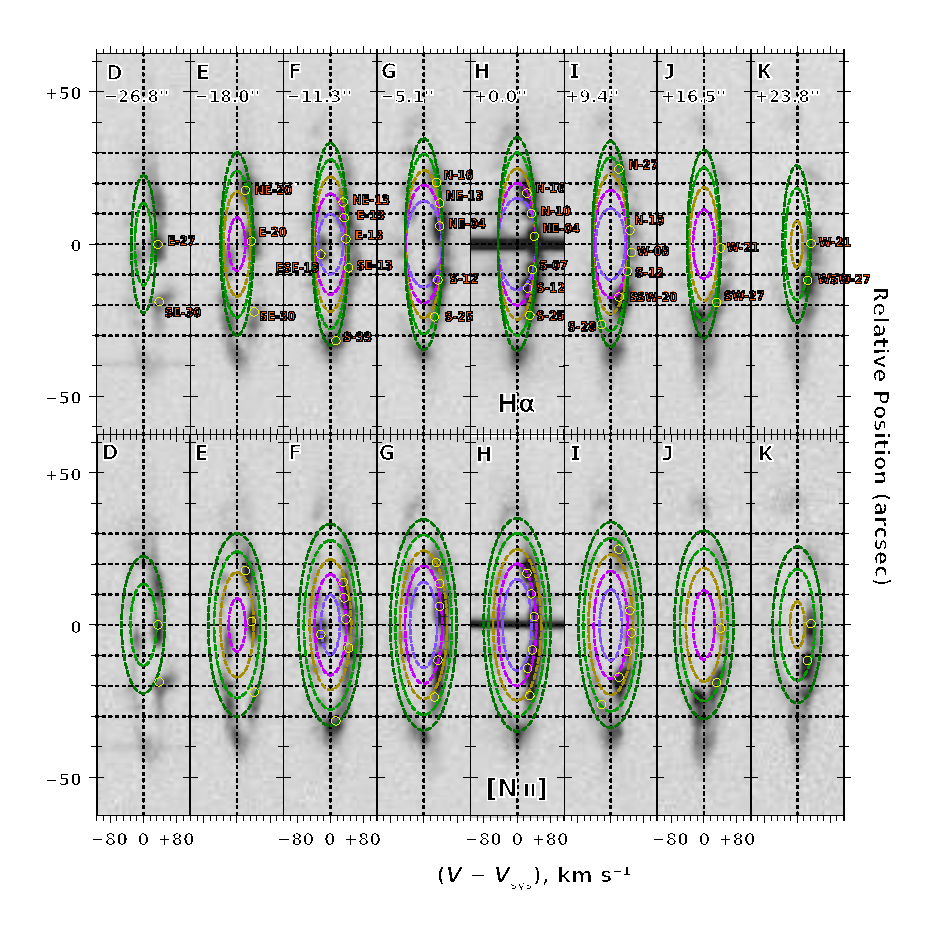
\includegraphics[width=\linewidth]{figs/zavala-slit-spectra-select-annotated}
  \caption{Kinematics of knot groups}
  \label{fig:longslit-spectra}
\end{figure}

\section{Conclusions}
\label{sec:conclusions}

\begin{acknowledgments}
  Thank you.
\end{acknowledgments}

\facilities{HST; JWST}

\bibliography{wr-globules-refs}

\end{document}

%%% Local Variables:
%%% mode: latex
%%% TeX-master: t
%%% End:
